\section[对称性和守恒定律]{对称性和守恒定律} \label{sec:03.10} % 
% \makebox[5em][s]{} % 短题目拉间距

物理学中的守恒定律总是和某种对称性相联系.这个事实早在19世纪研究经典分析力学时就已被发现,但其重要性直到建立量子力学后才逐渐显示出来.研究一个物理体系的对称性有助于了解体系的总体性质,发掘出隐藏的守恒量.通常,由对称性的研究得到的结论与求解薛定谔方程所得结论是等价的,而对称性的研究总是有助于薛定谔方程的求解.

设体系的总能量(哈密顿量)算符$\hat{H}$不随时间变化.体系的任何一个可以实现的运动状态,其波函数$\varPsi(\boldsymbol{r},t)$应该满足薛定谔方程
\begin{empheq}{equation}\label{eq310.1}
	i\hbar\frac{\partial}{\partial t}\varPsi=\hat{H}\varPsi
\end{empheq}
和归一化条件
\begin{empheq}{equation}\label{eq310.2}
	\int\varPsi^{*}\varPsi d\tau=1
\end{empheq}
以线性算符$T$表示施加于体系的某种物理变换(如平移,转动,等等),在此变换下任何状态$\varPsi$变成$T\varPsi$.如$T\varPsi$总也是体系的可以实现的状态,试问算符$T$应该具有什么性质,它与$H$之间应该具有何种关系?首先,$T\varPsi$应该满足归一化条件,即
\begin{empheq}{equation*}
	\int(T\varPsi)^{*}(T\varPsi)d\tau=1
\end{empheq}
由此容易证明(请读者自已完成)$T^{+}T=1$,即$T$为么正变换.其次,功应该满足薛定谔方程,即
\begin{empheq}{equation*}
	i\hbar\frac{\partial}{\partial t}(T\varPsi)=H(T\varPsi)
\end{empheq}
以$T^{+}$(即$T^{-1}$)作用上式,得到(设变换$T$与时间无关)
\begin{empheq}{equation*}
	i\hbar\frac{\partial}{\partial t}\varPsi=T^{+}HT\varPsi
\end{empheq}
与\eqref{eq310.1}式比较,即得
\begin{empheq}{equation}\label{eq310.3}
	T^{+}HT=H,\quad\text{即}\quad HT=TH
\end{empheq}
结论是:$T$为么正算符,并与总能量算符$H$对易.这种性质的变换,称为体系的对称性变换.如$T$已经是厄密的($T^{+}=T$),则$T$就是守恒量.如$T^{+}\neq T$,根据$T$的么正性,我们总可以将它表示成
\begin{empheq}{equation}\label{eq310.4}
	T=e^{i\lambda\hat{G}}
\end{empheq}
$\lambda$为实参数,$\hat{G}$为厄密算符,因此代表某种守恒量.简言之,找到了体系的一种对称性变换,也就找到了某种守恒量.

对称性变换可以是分立变换(例如空间反射),也可以是连续变换.连续变换的基础是无穷小变换
\begin{empheq}{equation}\label{eq310.5}
	T=1+i\varepsilon\hat{G}\quad(\varepsilon\rightarrow 0)
\end{empheq}
相当于\eqref{eq310.4}式中$\lambda\rightarrow\varepsilon$.根据么正条件,
\begin{empheq}{align*}
	T^{*}T&=(1-\varepsilon\hat{G}^{})(1+i\varepsilon\hat{G})	\\
	\approx& 1+i\varepsilon(\hat{G}\-\hat{G}^{+})=1
\end{empheq}
(略去$\varepsilon^{2}$项)可得
\begin{empheq}{equation}\label{eq310.6}
	\hat{G}=\hat{G}^{+}
\end{empheq}
即$\hat{G}$为厄密算符.而由\eqref{eq310.6}式可知$\hat{G}$应与$\hat{H}$对易,所以$\hat{G}$代表某种守恒量.$G$又称变换\eqref{eq310.5}的无穷小算子.

下面讨论几种重要的例子.

{\heiti 1. 空间反射不变性和宇称守恒定律}

定义空间反射变换$\hat{P}$,其作用规则为
\begin{empheq}{equation}\label{eq310.7}
	\hat{P}\varPsi(\boldsymbol{r},t)=\varPsi(-\boldsymbol{r},t)
\end{empheq}
$\hat{P}$也称宇称算符.显然,任何状态经过二次反射变换都应还原,即$\hat{P}^{2}$为恒等变换,由此可知
\begin{empheq}{equation}\label{eq310.8}
	\hat{P}^{2}=1,\quad \hat{P}^{+}=\hat{P}^{-1}=\hat{P}
\end{empheq}
$\hat{P}$的本征值$\lambda$显然也应满足$\lambda^{2}=1$,因此$\lambda=\pm 1$,相应的本征态为偶宇称态
($\lambda=1$)和奇宇称态($\lambda=-1$).

如体系的总能量算符$\hat{H}$具有空间反射不变性:
\begin{empheq}{equation}\label{eq310.9}
	\hat{P}\hat{H}=\hat{H}\hat{P},\quad \hat{P}^{+}\hat{H}\hat{P}=\hat{H}	
\end{empheq}
则$\hat{P}$为守恒量,这就是宇称守恒定律.在$\hat{H}$可以表示成
\begin{empheq}{equation}\label{eq310.10}
	\hat{H}=\hat{T}+\hat{V}=-\frac{\hbar^{2}}{2m}\nabla^{2}+V(\boldsymbol{r})
\end{empheq}
的情形,动能算符$\hat{T}$总是反射不变的,因此\eqref{eq310.9}式成立的条件是$V(-\boldsymbol{r})=V(\boldsymbol{r})$,即势能具有反射不变性.

{\heiti 2. 平移不变性和动量守恒定律}

先考虑一维问题.以$\hat{D}(a)$表示将体系平移距离$a$,体系的任何一个状态$\varPsi$经过平移,变成$\varPsi^{\prime}$,(图\ref{fig.3-4})波函数$\varPsi$,$\varPsi^{\prime}$的关系是
\pskip
\begin{wrapfigure}[8]{r}{9em}
	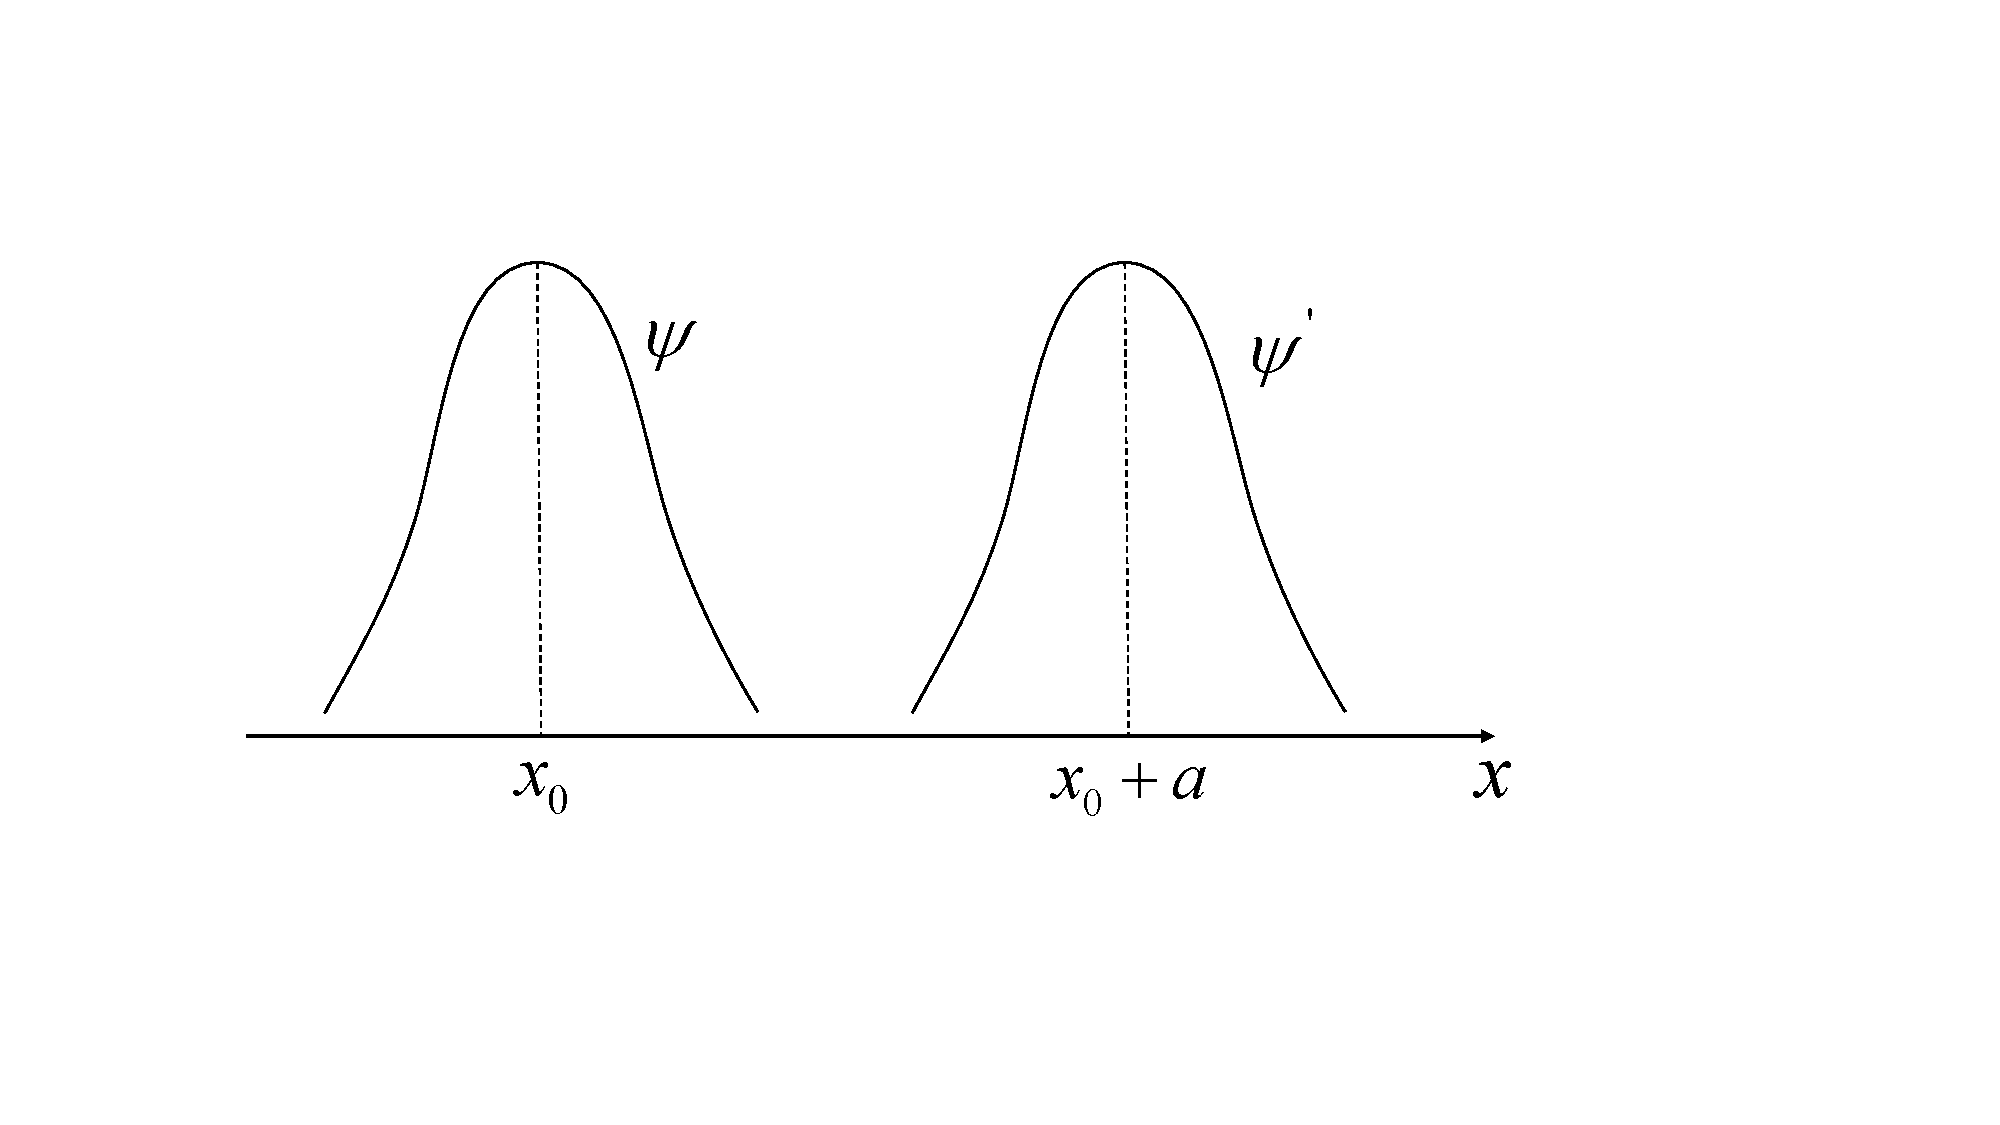
\includegraphics[width=3.5cm,clip]{QM file/figure/3-4}
	\caption{}\label{fig.3-4}
\end{wrapfigure}
\begin{empheq}{equation*}
	\varPsi^{\prime}(x)=\hat{D}(a)\varPsi(x)
\end{empheq}
显然
\begin{empheq}{equation*}
	\varPsi^{\prime}(x+a)=\varPsi(x)
\end{empheq}
因此
\begin{empheq}{equation}\label{eq310.11}
	\varPsi^{\prime}(x)=\hat{D}(a)\varPsi(x)=\varPsi(x-a)
\end{empheq}
这就是平移算符$\hat{D}(a)$对波函数的作用规则.平移显然是一种连续变换.我们先来确定无穷小平移$(a=\delta x\rightarrow 0)$算符$\hat{D}(\delta x)$)的具体形式.按照定义\eqref{eq310.11}式,应有
\eqindent{6}
\begin{empheq}{align*}
	\hat{D}(\delta x)\varPsi(x)&=\varPsi(x-\delta x)	\\
	&=\varPsi(x)-\frac{\partial \varPsi}{\partial x}\delta x=\bigg(1-\delta x\frac{\partial}{\partial x}\bigg)\varPsi(x)
\end{empheq}
所以
\begin{empheq}{align}\label{eq310.12}
	\hat{D}(\delta x)&=1-\delta x\frac{\partial}{\partial x}=1+\delta x\frac{\hat{p}_{x}}{i\hbar}	\nonumber\\
	&=\exp\bigg(\delta x\frac{\hat{p}_{x}}{i\hbar}\bigg)\quad(\delta x\rightarrow 0)
\end{empheq}
其中$\hat{p}_{x}$是动量算符.平移有限距离$a$时,算符$\hat{D}(a)$显然可以表示成
\begin{empheq}{equation}\label{eq310.13}
	\hat{D}(a)=\exp\bigg(-a\frac{\partial}{\partial x}\bigg)=\exp\bigg(a\hat{p}_{x}{i\hbar}\bigg)
\end{empheq}\eqnormal
将其代入\eqref{eq310.11}式,即得
\begin{empheq}{align*}
	\varPsi(x-a)=\exp\bigg(-a\frac{\partial}{\partial x}\bigg)\varPsi(x)	\\
	\sum_{n=0}^{\infty}\frac{(-a)^{n}}{n!}\bigg(\frac{\partial}{\partial x}\bigg)^{n}\varPsi(x)
\end{empheq}
这正是$\varPsi(x-a)$的泰勒(Taylor)展开式.

由以上分析,可知平移确是一种么正变换,满足
\eqindent{6}
\begin{equation}\label{eq310.14}
	\hat{D}^{+}(a)=\exp\bigg(\frac{ia}{\hbar}\hat{p}_{x}\bigg)=\hat{D}^{-1}(a)=\hat{D}(-a)
\end{equation}\eqnormal
其无穷小算子就是动量算符$\hat{p}_{x}$.

如体系的总能量算符$\hat{H}$具有平移不变性,满足
\begin{equation}\label{eq310.15}
	\hat{D}(a)\hat{H}=\hat{H}\hat{D}(a)
\end{equation}
则$\hat{H}$必与$\hat{p}_{x}$对易,即
\begin{empheq}{equation}\label{eq310.16}
	[\hat{p}_{x},\hat{H}]=\hat{p}_{x}\hat{H}-\hat{H}\hat{p}_{x}=0
\end{empheq}
$\hat{p}_{x}$为守恒量,这就是动量守恒定律.对于$\hat{H}$取
\begin{empheq}{equation*}
	\hat{H}=\hat{T}+\hat{V}=-\frac{\hbar^{2}}{2m}\frac{\partial^{2}}{\partial x^{2}}+V(x)
\end{empheq}
的情形,平移不变性要求$[V,p_{x}]$,则
\begin{empheq}{equation*}
	\frac{\partial V}{\partial x}=0,\quad V(x)=c\text{(常量)}
\end{empheq}
在这条件下,体系的动量守恒.经典力学也有同样的结论.

推广到三维问题,对于无限小平移$\delta r=(\delta x,\delta y,\delta z)$,相应的平移算符记为$\hat{D}(\delta \boldsymbol{r})$,应该有
\eqindent{6}
\begin{empheq}{align*}
	\hat{D}(\delta \boldsymbol{r})\varPsi(\boldsymbol{r})&=\varPsi(\boldsymbol{r}-\delta\boldsymbol{r})	\\
	&=\varPsi(\boldsymbol{r})-\bigg(\frac{\partial\varPsi}{\partial x}\delta x+\frac{\partial\varPsi}{\partial y}\delta y+\frac{\partial\varPsi}{\partial z}\delta z\bigg)	\\
	&=\varPsi(\boldsymbol{r})\sim\delta\boldsymbol{r}\cdot\nabla\varPsi
\end{empheq}
所以
\begin{empheq}{align}\label{eq310.17}
	\hat{D}(\delta \boldsymbol{r})&=1-\delta \boldsymbol{r}\cdot\nabla=\exp(-\delta \boldsymbol{r}\cdot\nabla)	\nonumber\\
	&=\exp\bigg(\delta \boldsymbol{r}\cdot\frac{\hat{\boldsymbol{p}}}{i\hbar}\bigg)(\delta \boldsymbol{r}\rightarrow 0)
\end{empheq}\eqnormal
其中$\hat{p}=-i\hbar\nabla$为动量算符.

平移有限距离$\boldsymbol{a}$时,算符$\hat{D}(\boldsymbol{a})$可以表示成
\begin{empheq}{equation}\label{eq310.18}
	\hat{D}(\boldsymbol{a})=\exp(-\boldsymbol{a}\cdot\nabla)=\exp\bigg(\boldsymbol{a}\cdot\frac{\hat{\boldsymbol{p}}}{i\hbar}\bigg)
\end{empheq}
如体系总能量算符$\hat{H}$具有平移不变性,满足
\begin{empheq}{equation}\label{eq310.19}
	\hat{D}(\boldsymbol{a})\hat{H}=\hat{H}\hat{D}(\boldsymbol{a})
\end{empheq}
则$\boldsymbol{a}\cdot\hat{\boldsymbol{p}}=a\hat{p}_{a}$必与$\hat{H}$对易,$\hat{p}_{a}$为守恒量.如上式对任意$\boldsymbol{a}$成立,则
\eqindent{6}
\begin{empheq}{equation}\label{eq310.20}
	[\hat{p}_{\alpha},\hat{H}]=\hat{p}_{\alpha}\hat{H}-\hat{H}\hat{p}_{\alpha}=0,\quad\alpha=x,y,z
\end{empheq}\eqnormal
$\boldsymbol{p}$为守恒量,这就是动量守恒定律.$\hat{H}$取\eqref{eq310.10}式时,平移不变性要求$[V,\hat{p}_{\alpha}]=0(\alpha=x,y,z)$,则
\begin{empheq}{equation*}
	\frac{\partial V}{\partial x},\frac{\partial V}{\partial y}=0,\frac{\partial V}{\partial z}=0,V(\boldsymbol{r})=c\text{(常量)}
\end{empheq}
在这条件下,体系的动量守恒.

{\heiti 3. 旋转不变性和角动量守恒定律}

考虑体系绕任意轴$\boldsymbol{e}_{n}$的旋转,对于无穷小旋转角$\delta\varphi$,相应的转动算符记为$\hat{R}(\delta\varphi)$,$\delta\varphi=\boldsymbol{e}_{n}\delta\varphi$.体系的任何一个状态$\varPsi$,经无限小转动后,变成$\varPsi^{\prime}$,即$\hat{R}(\delta\varphi)\varPsi$,它与$\varPsi$的关系可以仿照平移变换而确定.先考虑一种简单情形,即转轴为球坐标系极轴($z$轴)的情形.令$\hat{R}(\delta\varphi)\varPsi=\varPsi^{\prime}$,显然有
\eqindent{4}
\begin{empheq}{align*}
	\varPsi^{\prime}(r,\theta,\varphi)&=\hat{R}(\delta\varphi)\varPsi(r,\theta,\varphi)=\varPsi(r,\theta,\varphi-\delta\varphi)	\\
	&=\varPsi(r,\theta,\varphi)-\frac{\partial\varPsi}{\partial\varphi}\delta\varphi=\bigg(1-\delta\varphi\frac{\partial}{\partial\varphi}\bigg)\varPsi(r,\theta,\varphi)
\end{empheq}\eqnormal

\begin{wrapfigure}[14]{r}{5em}
	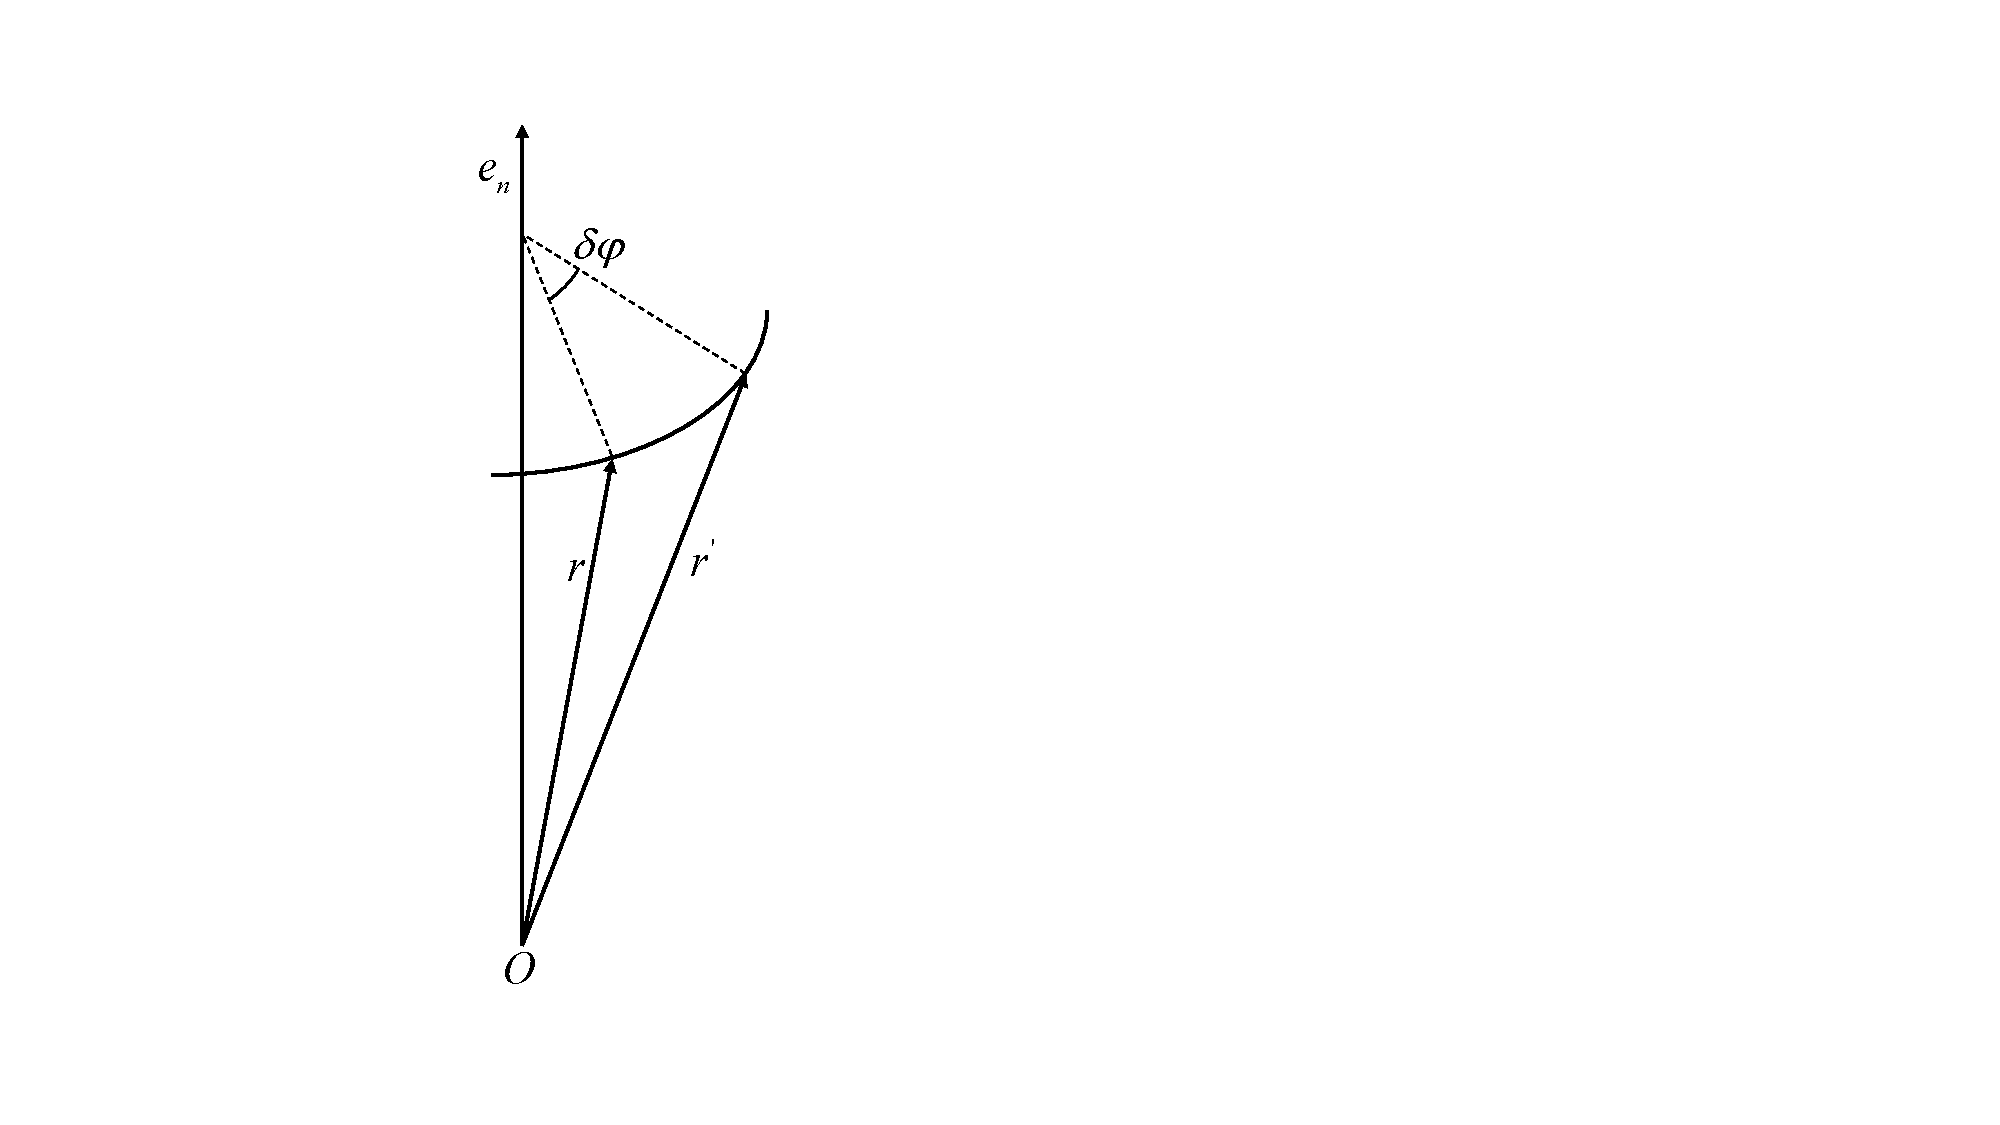
\includegraphics[width=2cm,clip]{QM file/figure/3-5}
	\caption{}\label{fig.3-5}
\end{wrapfigure}
所以
\eqindent{4}
\begin{empheq}{align}\label{eq310.21}
	\hat{R}(\delta\varphi)&=1-\delta\varphi\frac{\partial}{\partial\varphi}=1+\delta\varphi\frac{\hat{L}_{z}}{i\hbar}	\nonumber\\
	&=\exp\bigg(\delta\varphi\frac{\hat{L}_{z}}{i\hbar}\bigg)
\end{empheq}\eqnormal
其中
\eqindent{6}
\begin{empheq}{equation}\label{eq310.22}
	\hat{L}_{z}=-i\hbar\frac{\partial}{\partial\varphi}
\end{empheq}
为转动变换的无穷小算子,这就是轨道角动量($z$分量)算符.

当旋转轴$\boldsymbol{e}_{n}$沿任意方向时,矢径$\boldsymbol{r}$经过无穷小转动后变成(图\ref{fig.3-5})
\begin{empheq}{equation}\label{eq310.23}
	\boldsymbol{r}^{\prime}=\boldsymbol{r}+\delta\boldsymbol{r},\quad\delta\boldsymbol{r}=\delta\varphi\boldsymbol{e}_{n}\times\boldsymbol{r}
\end{empheq}
转动前后波函数关系为
\begin{empheq}{equation}\label{eq310.24}
	\varPsi^{\prime}(\boldsymbol{r}^{\prime})=\varPsi(\boldsymbol{r})
\end{empheq}
\begin{empheq}{align*}
	\varPsi^{\prime}(\boldsymbol{r})&=\hat{R}(\delta\varphi)\varPsi(\boldsymbol{r})=\varPsi(\boldsymbol{r}-\delta\boldsymbol{r})	\\
	&=\varPsi(\boldsymbol{r})-\delta\boldsymbol{r}\cdot\nabla\varPsi(\boldsymbol{r})=(1-\delta\boldsymbol{r}\cdot\nabla)\varPsi(\boldsymbol{r})	\\
	&=[1-\delta\varphi(\boldsymbol{e}_{n}\times\boldsymbol{r})\cdot\nabla]\varPsi(\boldsymbol{r})	\\
	&=[1-\delta\varphi\boldsymbol{e}_{n}\cdot(\boldsymbol{r}\times\nabla)]\varPsi(\boldsymbol{r})
\end{empheq}
所以
\begin{empheq}{align}\label{eq310.25}
	\hat{R}(\delta\varphi)&=1-\delta\varphi\boldsymbol{e}_{n}\cdot(\boldsymbol{r}\times\nabla)	\nonumber\\
	&=1+\frac{\delta\varphi}{i\hbar}\boldsymbol{e}_{n}\cdot\hat{\boldsymbol{L}}
	=\exp\bigg(\frac{\delta\varphi}{i\hbar}\boldsymbol{e}_{n}\cdot\hat{\boldsymbol{L}}\bigg)
\end{empheq}\eqnormal
其中
\begin{empheq}{equation}\label{eq310.26}
	\hat{\boldsymbol{L}}=-i\hbar\boldsymbol{r}\times\nabla=\boldsymbol{r}\times\hat{\boldsymbol{p}}
\end{empheq}
是轨道角动量算符,$\boldsymbol{e}_{n}\cdot\hat{\boldsymbol{L}}=\hat{L}_{n}$是转动变换的无穷小算子.

如体系具有对$\boldsymbol{e}_{n}$轴的旋转不变性,满足
\begin{empheq}{equation}\label{eq310.27}
	\hat{R}(\delta\varphi)\hat{H}=\hat{H}\hat{R}(\delta\varphi)
\end{empheq}
则$\hat{L}_{n}$与$\hat{H}$必然对易,即
\begin{empheq}{equation}\label{eq310.28}
	[\hat{L}_{n},\hat{H}]=\hat{L}_{n}\hat{H}-\hat{H}\hat{L}_{n}=0
\end{empheq}
$L_{n}$为守恒量.如$\hat{H}$具有对任意轴的旋转不变性,则$\hat{\boldsymbol{L}}$各分量均与$\hat{H}$对易,即
\begin{empheq}{equation}\label{eq310.29}
	[\hat{L}_{\alpha},\hat{H}]=\hat{L}_{\alpha}\hat{H}-\hat{H}\hat{L}_{\alpha}=0,\quad\alpha=x,y,z
\end{empheq}
$\boldsymbol{L}$为守恒量.在$\hat{H}$可以表示成\eqref{eq310.10}式的情形下,动能算符$\hat{T}=-\frac{\hbar^{2}}{2m}\nabla^{2}$具有对任意轴的旋转不变性,满足
\begin{empheq}{equation}\label{eq310.30}
	[\hat{L}_{\alpha},\hat{T}]=0,\quad\alpha=x,y,z
\end{empheq}
因此势能$V(r)$具有哪种旋转对称性,$\hat{H}$也具有同样的对称性.例如中心力场,$V=V(r)$,满足
\begin{empheq}{equation}\label{eq310.31}
	[\hat{L}_{\alpha},V(r)]=0,\quad\alpha=x,y,z
\end{empheq}
$V(r)$各向同性,具有对任意轴的旋转不变性,$\hat{H}$也一样,因此$\boldsymbol{L}$为守恒量,这就是角动量守恒定律.

{\heiti 4. 时间平移不变性和能量守恒定律}

在$\S$中\ref{sec:03.09}已经讲过,如体系的哈密顿算符$\hat{H}$不显含$t$,$\hat{H}$就是守恒量,这就是能量守恒定律.$\hat{H}$不显含$t$,意味着体系具有时间均匀性,体系能量不随时间变化,$\frac{\partial\hat{H}}{\partial t}$.当然,在量子力学中,时间$t$并不作为力学量对待,但是我们仍然可以仿照空间平移的概念,引入时间平移概念.任何状态$\varPsi(\boldsymbol{r},t)$的无穷小时间$(\delta t)$平移态记为$D_{t}(\delta t)\varPsi$,它在$t$时刻的情况与$\varPsi$态$(t+\delta t)$时刻的情况相同,即
\begin{empheq}{equation}\label{eq310.32}
	D_{t}(\delta t)\varPsi(\boldsymbol{r},t)=\varPsi(\boldsymbol{r},t+\delta t)
\end{empheq}
由于
\begin{empheq}{equation*}
	\varPsi(\boldsymbol{r},t+\delta t)=\varPsi(\boldsymbol{r},t)+\delta t\frac{\partial}{\partial t}\varPsi(\boldsymbol{r},t)
\end{empheq}
所以无穷小时间平移算符为
\begin{empheq}{equation}\label{eq310.33}
	D_{t}(\delta t)=1+\delta t\frac{\partial}{\partial t}=\exp\bigg(\delta t\frac{\partial}{\partial t}\bigg)
\end{empheq}
有限时间$(\tau)$平移算符为
\begin{empheq}{equation}\label{eq310.34}
	D_{t}(\tau)=\exp\bigg(\tau\frac{\partial}{\partial t}\bigg)
\end{empheq}
任何真实的运动状态$\varPsi(\boldsymbol{r},t)$应该满足薛定谔方程\eqref{eq310.1}式,$\frac{\partial}{\partial t}$对波函数的作用效果等价于$\frac{\hat{H}}{i\hbar}$,所以在时间平移算符中,可作如下等价代换:
\begin{empheq}{equation}\label{eq310.35}
	i\hbar\frac{\partial}{\partial t}\Longrightarrow\hat{H}
\end{empheq}
\begin{empheq}{equation}\label{eq310.36}
	D_{t}(\tau)\Longrightarrow\exp\bigg(\frac{\tau\hat{H}}{i\hbar}\bigg)
\end{empheq}
\eqref{eq310.35}式的含义正是$\S$\ref{sec:02.01}就已经讲过的,$i\hbar\frac{\partial}{\partial t}$代表能量.而\eqref{eq310.36}式表明,时间平移算符等价于演化算符[参看\eqref{eq39.7}式].

体系在时间上的均匀性也称时间平移不变性,这种对称性导致能量守恒定律成立.但应注意,这并不意味若体系在任何时刻必定处于能量本征态.这里“能量守恒”的确切内容是体系的能量平均值以及各个能量本征值的测量概率不随时间改变.以$\varPsi(\boldsymbol{r})$表示$\hat{H}$的本征态,本征值记为$E_{n}$.如在初始时刻$(t_{0}=0)$体系处于能量本征态$\varPsi_{n}$,波函数的时间演化规律为
\begin{empheq}{equation}\label{eq310.37}
	\varPsi_{n}(\boldsymbol{r},t)=\varPsi_{n}(\boldsymbol{r})e^{-E_{n}t/i\hbar}
\end{empheq}
这就是定态波函数.上式的时间平移$(\tau)$态为
\eqindent{6}
\begin{empheq}{align}\label{eq310.38}
	D_{t}\varPsi_{n}(\boldsymbol{r},t)&=e^{\tau\frac{\partial}{\partial t}}\varPsi_{n}(\boldsymbol{r})e^{-iE_{n}t/\hbar}	\nonumber\\
	&=\varPsi_{n}(\boldsymbol{r})\exp\bigg[-\frac{i}{\hbar}E_{n}(t+\tau)\bigg]
\end{empheq}\eqnormal
仍是原来的定态,只是添了相因子$\exp\bigg(-\frac{i}{\hbar}E_{n}(t+\tau)\bigg)$.如初始状态不是单一的能量本征态,则总可以表示成各$\varPsi_{n}$的线性叠加:
\begin{empheq}{equation}\label{eq310.39}
	\varPsi(\boldsymbol{r},t)=\sum_{n}C_{n}\varPsi_{n}(\boldsymbol{r})
\end{empheq}
波函数的时间演化规律为[\eqref{eq39.6}式]
\begin{empheq}{align}\label{eq310.40}
	\varPsi(\boldsymbol{r},0)&=\exp\bigg(\frac{\hat{H}t}{i\hbar}\bigg)\varPsi(\boldsymbol{r},0)	\nonumber\\
	&=\sum_{n}C_{n}\varPsi_{n}(\boldsymbol{r})e^{-E_{n}t/\hbar}
\end{empheq}
上式的时间平移$(\tau)$态为
\eqindent{6}
\begin{empheq}{align}\label{eq310.41}
	D_{t}(\tau)\varPsi(\boldsymbol{r},t)&=\exp\bigg(\frac{\hat{H}\tau}{i\hbar}\bigg)\varPsi(\boldsymbol{r},t)	\nonumber\\
	&=\exp\bigg[\frac{\hat{H}(t+\tau)}{i\hbar}\bigg]\varPsi(\boldsymbol{r},0)	\nonumber\\
	&=\sum_{n}C_{n}\varPsi_{n}(\boldsymbol{r})\exp\bigg[-\frac{i}{\hbar}E_{n}(t+\tau)\bigg]	\nonumber\\
	&=\varPsi(\boldsymbol{r},t+\tau)
\end{empheq}\eqnormal
显然,无论是\eqref{eq310.40}式还是\eqref{eq310.41}式,能量本征值$E_{n}$的测量概率均为$|C_{n}|^{2}$,与时间$t$及$\tau$无关,而仅取决于初始状态$\varPsi(\boldsymbol{r},0)$.

\example 质量为$m$的粒子作三维运动,已知总能量算符为
\begin{empheq}{equation}\label{eq310.42}
	\hat{H}=\hat{T}+V=-\frac{\hbar^{2}}{2m}\nabla^{2}+\frac{k}{2}(x^{2}+y^{2})
\end{empheq}
试分析其对称性并找出相应的守恒量.

\solution 首先,$\hat{H}$不显含$t$,具有时间均匀性,$H$为守恒量(能量守恒).$H_{x}=\frac{p_{x}^{2}}{2m}+\frac{kx^{2}}{2}$,$H_{y}=\frac{p_{y}^{2}}{2m}+\frac{ky^{2}}{2}$和$H_{z}=\frac{p_{z}^{2}}{2m}+\frac{kz^{2}}{2}$也都是守恒量.

其次,$\hat{H}$显然具有空间反射不变性,所以宇称守恒.

由于势能$V$与$z$无关,$\hat{H}$具有$z$方向平移不变性,所以动量的$z$分量$p_{z}$是守恒量.

势能$V$还具有绕$z$轴的旋转不变性,$\frac{\partial V}{\partial\varphi}$,所以轨道角动盘的$z$分量$L_{z}$,也是守恒量.






